\documentclass[12pt,a4paper]{article}

% ─── Page Layout ───────────────────────────────────────────────────────────────
\usepackage[a4paper, margin=0.8in, headheight=14pt]{geometry}

% ─── Fonts (XeLaTeX) ───────────────────────────────────────────────────────────
\usepackage{fontspec}
\usepackage{unicode-math}
\setmainfont{TeX Gyre Pagella}
\setmonofont[Scale=0.88]{TeX Gyre Cursor}
\setmathfont{Latin Modern Math}

% ─── Packages ──────────────────────────────────────────────────────────────────
\usepackage{xcolor}
\usepackage{colortbl}
\usepackage{titlesec}
\usepackage{enumitem}
\usepackage{tabularx}
\usepackage{booktabs}
\usepackage{array}
\usepackage{amsmath}
\usepackage{tikz}
\usetikzlibrary{shapes.geometric, arrows.meta, positioning, calc, fit, decorations.pathreplacing}
\usepackage{tcolorbox}
\tcbuselibrary{skins, breakable}
\usepackage{hyperref}
\usepackage{fancyhdr}
\usepackage{graphicx}
\usepackage{microtype}
\hyphenpenalty=10000
\exhyphenpenalty=10000
\sloppy
\usepackage{caption}
\usepackage{setspace}
\usepackage{multirow}
\usepackage{tocloft}

% ─── Q&A helper ────────────────────────────────────────────────────────────────
\newcommand{\Q}[1]{\textbf{#1}\par\noindent\ignorespaces}

% ─── Colour Palette ────────────────────────────────────────────────────────────
\definecolor{myred}{RGB}{196,30,58}
\definecolor{mydark}{RGB}{30,30,50}
\definecolor{mygreen}{RGB}{14,120,80}
\definecolor{myteal}{RGB}{0,130,140}
\definecolor{myamber}{RGB}{180,100,0}
\definecolor{mypurple}{RGB}{100,30,160}
\definecolor{mygray}{RGB}{246,247,249}
\definecolor{mgframe}{RGB}{180,185,200}
\definecolor{watermark}{RGB}{145,150,170}
\definecolor{hdrred}{RGB}{250,232,235}
\definecolor{hdrgreen}{RGB}{220,244,233}
\definecolor{hdrteal}{RGB}{220,242,244}
\definecolor{hdramber}{RGB}{253,242,215}
\definecolor{hdrpurple}{RGB}{238,228,255}
\definecolor{hdrgray}{RGB}{238,240,245}
\definecolor{rowalt}{RGB}{250,251,253}

% ─── Section Formatting ────────────────────────────────────────────────────────
\titleformat{\section}
  {\large\bfseries\color{myred}}{\thesection.}{0.5em}{}
  [\vspace{1pt}{\color{myred}\rule{\linewidth}{0.8pt}}]
\titleformat{\subsection}
  {\normalsize\bfseries\color{myteal}}{\thesubsection}{0.5em}{}
\titlespacing*{\section}{0pt}{18pt}{7pt}
\titlespacing*{\subsection}{0pt}{11pt}{4pt}

% ─── Paragraph ─────────────────────────────────────────────────────────────────
\setlength{\parindent}{0pt}
\setlength{\parskip}{4pt}

% ─── TOC Styling ───────────────────────────────────────────────────────────────
\renewcommand{\cfttoctitlefont}{\large\bfseries\color{myred}}
\renewcommand{\cftaftertoctitle}{\par\noindent{\color{myred}\rule{\linewidth}{0.8pt}}}
\setlength{\cftbeforetoctitleskip}{0pt}
\setlength{\cftaftertoctitleskip}{6pt}
\renewcommand{\cftsecfont}{\normalsize\bfseries\color{mydark}}
\renewcommand{\cftsecpagefont}{\normalsize\bfseries\color{mydark}}
\renewcommand{\cftsecleader}{\cftdotfill{\cftdotsep}}
\setlength{\cftbeforesecskip}{7pt}
\renewcommand{\cftsubsecfont}{\small\color{mydark}}
\renewcommand{\cftsubsecpagefont}{\small\color{mydark}}
\setlength{\cftbeforesubsecskip}{3pt}
\setlength{\cftsubsecindent}{1.4em}

% ─── Table helpers ─────────────────────────────────────────────────────────────
\renewcommand{\arraystretch}{1.45}
\setlength{\tabcolsep}{6pt}
\arrayrulecolor{mydark}
\newcolumntype{B}[1]{>{\small\bfseries\raggedright\arraybackslash}m{#1}}
\newcolumntype{Y}{>{\small\raggedright\arraybackslash}X}
\renewcommand{\tabularxcolumn}[1]{m{#1}}

% ─── Header / Footer ───────────────────────────────────────────────────────────
\pagestyle{fancy}
\fancyhf{}
\fancyhead[L]{\small\color{myred}\textbf{EC501}\;\color{mydark}--- Electromagnetic Waves}
\fancyhead[R]{\small\color{myteal}\textbf{Module 5 Notes}}
\fancyfoot[C]{\small\color{mydark}\thepage}
\fancyfoot[R]{\small\color{watermark}\textit{\copyright\ Biraj}}
\renewcommand{\headrulewidth}{0.5pt}
\renewcommand{\footrulewidth}{0.3pt}

% ─── Hyperref ──────────────────────────────────────────────────────────────────
\hypersetup{
  colorlinks=true, linkcolor=myteal, urlcolor=myteal,
  pdfauthor={Biraj Sarkar},
  pdftitle={EC501 --- Module 5 Notes}
}

% ─── tcolorbox styles ──────────────────────────────────────────────────────────
\tcbset{
  tikzbox/.style={
    colback=mygray, colframe=mgframe, boxrule=0.6pt, arc=4pt,
    left=8pt, right=8pt, top=6pt, bottom=6pt,
    colbacktitle=mgframe, coltitle=mydark,
    fonttitle=\small\bfseries
  },
  defbox/.style={
    colback=hdrgreen, colframe=mygreen, boxrule=0.8pt, arc=4pt,
    left=9pt, right=9pt, top=6pt, bottom=6pt,
    colbacktitle=mygreen, coltitle=white,
    fonttitle=\small\bfseries
  },
  formulabox/.style={
    colback=hdrteal, colframe=myteal, boxrule=0.8pt, arc=4pt,
    left=9pt, right=9pt, top=7pt, bottom=7pt,
    colbacktitle=myteal, coltitle=white,
    fonttitle=\small\bfseries
  },
  examplebox/.style={
    colback=hdramber, colframe=myamber, boxrule=0.8pt, arc=4pt,
    left=9pt, right=9pt, top=6pt, bottom=6pt,
    colbacktitle=myamber, coltitle=white,
    fonttitle=\small\bfseries
  },
  masonbox/.style={
    colback=hdrpurple, colframe=mypurple, boxrule=0.8pt, arc=4pt,
    left=9pt, right=9pt, top=6pt, bottom=6pt,
    colbacktitle=mypurple, coltitle=white,
    fonttitle=\small\bfseries
  },
  exambox/.style={
    colback=hdrpurple, colframe=mypurple, boxrule=1pt, arc=5pt,
    left=10pt, right=10pt, top=8pt, bottom=8pt,
    colbacktitle=mypurple, coltitle=white,
    fonttitle=\bfseries,
    breakable, title after break={\textbf{Frequently Asked / Viva Questions (contd.)}}}
}
% Make all boxes breakable across pages
\tcbset{breakable}

% ─── TikZ styles ───────────────────────────────────────────────────────────────
\tikzset{
  block/.style={rectangle, draw=myteal, fill=hdrteal,
    text width=2.4cm, align=center, minimum height=0.95cm,
    font=\small, rounded corners=3pt, line width=0.7pt},
  redblock/.style={rectangle, draw=myred, fill=hdrred,
    text width=2.4cm, align=center, minimum height=0.95cm,
    font=\small, rounded corners=3pt, line width=0.7pt},
  netnode/.style={rectangle, draw=myteal, fill=hdrteal,
    text width=1.5cm, align=center, minimum height=0.8cm,
    font=\small, rounded corners=3pt, line width=0.7pt},
  sumjunc/.style={circle, draw=myamber, fill=hdramber,
    minimum size=0.62cm, font=\small, line width=0.8pt},
  snode/.style={circle, draw=mypurple, fill=hdrpurple,
    minimum size=0.55cm, font=\footnotesize, line width=0.7pt},
  arrow/.style={-Stealth, thick, color=mydark},
  redarrow/.style={-Stealth, thick, color=myred},
  line/.style={thick, color=mydark}
}

% ═══════════════════════════════════════════════════════════════════════════════
\begin{document}
% ═══════════════════════════════════════════════════════════════════════════════

\begin{center}
  {\LARGE\bfseries\color{myred} EC501 --- Electromagnetic Waves}\\[5pt]
  {\normalsize\color{mydark} Semester V \quad$\bullet$\quad 3L:0T:0P \quad$\bullet$\quad 3 Credits}\\[3pt]
  {\normalsize\color{myteal}\textbf{Module 5 Exam Notes: Radiation and Antennas}}\\[3pt]
  {\small\color{mydark} CGEC \;$|$\; B.Tech ECE (2023--27) \;$|$\; \textit{Biraj Sarkar}}
\end{center}
\vspace{2pt}
\noindent{\color{myred}\rule{\linewidth}{1.5pt}}
\vspace{2pt}

\hypersetup{linkcolor=mydark}
\tableofcontents
\hypersetup{linkcolor=myteal}
\newpage

\section{Electromagnetic Potentials and Radiation}
\begin{tcolorbox}[defbox,title={Scalar and vector potentials}]
The vector potential $\mathbf A$ determines magnetic flux by $\mathbf B=\nabla\times\mathbf A$. The electric field is $\mathbf E=-\nabla\Phi-\partial_t\mathbf A$, where $\Phi$ is the scalar potential. Potentials are useful for finding the fields of localized charge and current distributions.
\end{tcolorbox}

Assume a uniform lossless medium, $v=1/\sqrt{\mu\epsilon}$, $k=\omega/v$, $\eta=\sqrt{\mu/\epsilon}$ and peak phasors with $e^{j\omega t}$. The potential representation satisfies magnetic Gauss law and Faraday's law. It allows the Lorenz gauge $\nabla\cdot\mathbf A=-j\omega\mu\epsilon\Phi$.
\subsection{Wave equations and their outgoing solutions}
Insert the potentials into Amp\`ere--Maxwell. Use $\nabla\times\nabla\times\mathbf A=\nabla(\nabla\cdot\mathbf A)-\nabla^2\mathbf A$:
\[
\begin{aligned}
\nabla(\nabla\cdot\mathbf A)-\nabla^2\mathbf A
 &=\mu\mathbf J-j\omega\mu\epsilon\nabla\Phi+k^2\mathbf A,\\
(\nabla^2+k^2)\mathbf A&=-\mu\mathbf J.
\end{aligned}
\]
Electric Gauss law gives $-\nabla^2\Phi-j\omega\nabla\cdot\mathbf A=\rho_v/\epsilon$, hence $(\nabla^2+k^2)\Phi=-\rho_v/\epsilon$. For an unbounded medium write $R=|\mathbf r-\mathbf r'|$:
\[
\begin{aligned}
\mathbf A(\mathbf r)&=\frac{\mu}{4\pi}\int_V
     \mathbf J(\mathbf r')\frac{e^{-jkR}}{R}\,dV',\\
\Phi(\mathbf r)&=\frac{1}{4\pi\epsilon}\int_V
     \rho_v(\mathbf r')\frac{e^{-jkR}}{R}\,dV'.
\end{aligned}
\]
Outside a point source the radial kernel solves the homogeneous Helmholtz equation. A small sphere about the source fixes the $1/(4\pi)$ factor by the flux integral. The outgoing sign follows because $\omega t-kR$ is a phase moving to larger $R$. In time domain each source is evaluated at the retarded time $t-R/v$.
\begin{itemize}[leftmargin=*,itemsep=3pt]
\item \textbf{Far-zone amplitude.} Use $1/R\approx1/r$ for $r$ much larger than the source size.
\item \textbf{Far-zone phase.} Keep $R\approx r-\hat{\mathbf r}\cdot\mathbf r'$ in the exponential. Discarding the second term can erase the directional pattern of an extended antenna.
\item \textbf{Field reconstruction.} The leading spatial derivative is $-jk\hat{\mathbf r}$. Thus $\mathbf H_{\rm far}\approx-jk\hat{\mathbf r}\times\mathbf A/\mu$ and $\mathbf E_{\rm far}\approx\eta\mathbf H_{\rm far}\times\hat{\mathbf r}$.
\end{itemize}

\section{Hertzian Dipole}
\begin{tcolorbox}[defbox,title={Hertzian dipole}]
A Hertzian dipole is an ideal electrically short current element of length $\ell\ll\lambda$, carrying uniform peak phasor current $I_0$. Its moment $I_0\ell$ is directed along the element.
\end{tcolorbox}

For an element at the origin along $z$, $\mathbf A=\hat{\mathbf z}\mu I_0\ell e^{-jkr}/(4\pi r)$. Use $\hat{\mathbf z}=\hat{\mathbf r}\cos\theta-\hat{\boldsymbol\theta}\sin\theta$.
\[
H_\phi=\frac{\partial_r(r A_\theta)-\partial_\theta A_r}{\mu r}
  =\frac{I_0\ell\sin\theta}{4\pi}e^{-jkr}
   \left(\frac{jk}{r}+\frac{1}{r^2}\right).
\]
Outside the source, $\mathbf E=(\nabla\times\mathbf H)/(j\omega\epsilon)$. Define $C=I_0\ell e^{-jkr}/(4\pi)$ at the field point. The nonzero electric components are
\[
\begin{aligned}
E_r&=2\eta C\cos\theta\left(\frac{1}{r^2}+\frac{1}{jk r^3}\right),\\
E_\theta&=\eta C\sin\theta\left(\frac{jk}{r}+\frac{1}{r^2}+\frac{1}{jk r^3}\right).
\end{aligned}
\]
The $1/r^3$ and $1/r^2$ terms matter in the near field. At $kr\gg1$ keep only $1/r$ terms: $E_\theta\approx\eta H_\phi=j\eta k I_0\ell\,e^{-jkr}\sin\theta/(4\pi r)$. The fields are transverse and in phase, with outward mean power. The axial direction is a null and broadside is maximum. The field is linearly polarized along $\hat{\boldsymbol\theta}$ away from nulls.
\begin{tcolorbox}[tikzbox,title={Hertzian dipole and normalized elevation-plane power pattern},unbreakable]
\centering
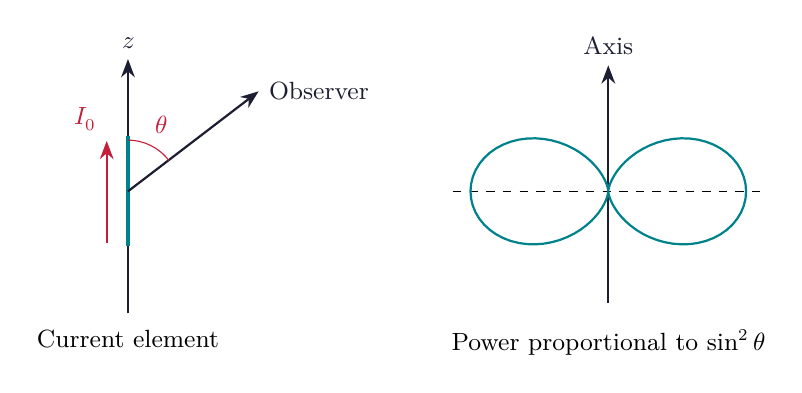
\begin{tikzpicture}[font=\small]
\draw[arrow] (0,-1.55)--(0,1.68) node[above] {$z$};
\draw[very thick,myteal] (0,-.7)--(0,.7);
\draw[redarrow] (-.27,-.66)--(-.27,.64) node[above left] {$I_0$};
\draw[arrow] (0,0)--(1.66,1.27) node[right] {Observer};
\draw[myred] (0,.65) arc (90:37:.65);
\node[myred] at (.42,.85) {$\theta$};
\node[below] at (0,-1.63) {Current element};
\begin{scope}[xshift=6.1cm]
\draw[arrow] (0,-1.42)--(0,1.6) node[above] {Axis};
\draw[dashed] (-1.97,0)--(1.97,0);
\draw[thick,myteal,domain=0:360,samples=121]
 plot ({1.75*sin(\x)^3},{1.75*sin(\x)^2*cos(\x)});
\node[below] at (0,-1.63) {Power proportional to $\sin^2\theta$};
\end{scope}
\end{tikzpicture}
\end{tcolorbox}
\subsection{Radiated power and radiation resistance}
Radiation intensity $U=r^2\langle S_r\rangle$ is power per solid angle, in $\mathrm{W/sr}$. In the radiation zone $\langle S_r\rangle=|E_\theta|^2/(2\eta)$. Integrate over a sphere:
\[
\begin{aligned}
U(\theta)&=\frac{\eta k^2|I_0\ell|^2}{32\pi^2}\sin^2\theta,\\
P_{\rm rad}&=\frac{\eta k^2|I_0\ell|^2}{32\pi^2}
 \int_0^{2\pi}d\phi\int_0^\pi\sin^3\theta\,d\theta\\
 &=\frac{\eta k^2|I_0\ell|^2}{12\pi}.
\end{aligned}
\]
The last integral is $4/3$ by substitution $u=\cos\theta$. With peak current $P_{\rm rad}=|I_0|^2R_r/2$, so $R_r=\eta k^2\ell^2/(6\pi)=80\pi^2(\ell/\lambda)^2\,\Omega$ in free space. Finally $D_0=4\pi U_{\max}/P_{\rm rad}=1.5=1.76\,\mathrm{dBi}$.
\begin{tcolorbox}[examplebox,title={Power from a current element}]
In free space, take $\ell=\lambda/20$ and $I_0=2\,\mathrm A$ peak. Then $R_r=80\pi^2/400=1.974\,\Omega$ and $P_{\rm rad}=(2^2/2)(1.974)=3.95\,\mathrm W$. The result is for uniform current. A physical short dipole of the same length with triangular current radiates less for the same feed current.
\end{tcolorbox}

\section{Antenna Parameters and Reception}
\begin{tcolorbox}[defbox,title={Radiation pattern and antenna gain}]
A radiation pattern describes directional variation of far field or power. Directivity compares radiation intensity with the average intensity over the sphere. Gain also accounts for power dissipated within the antenna.
\end{tcolorbox}
\subsection{Pattern, power and feed quantities}
\par\vspace{6pt}\noindent
\begin{tabularx}{\linewidth}{|B{3.9cm}|Y|}\hline
Parameter & Definition or formula \\ \hline
Directivity & $D(\theta,\phi)=4\pi U/P_{\rm rad}$. $D_0$ is its maximum. \\ \hline
Radiation efficiency and gain & $e_r=P_{\rm rad}/P_{\rm accepted}$ and $G=e_rD$. Realized gain further includes mismatch at the chosen port. \\ \hline
Beamwidth & Half-power beamwidth (HPBW) is the angle between the two $-3\,\mathrm{dB}$ points around a lobe. First-null beamwidth is the angle between the first nulls where both exist in that cut. \\ \hline
Input impedance & $Z_A=R_r+R_{\rm loss}+jX_A$. Resonance means $X_A=0$, while feed matching also depends on the real part. \\ \hline
Bandwidth & Frequency interval satisfying a stated criterion, such as acceptable voltage standing-wave ratio, gain or pattern. Fractional bandwidth is $(f_H-f_L)/f_0$. \\ \hline
Polarization & Direction and time trajectory of the far electric vector for a specified observation direction. \\ \hline
\end{tabularx}

For a Hertzian dipole, $\sin^2\theta=1/2$ at $45^\circ$ and $135^\circ$. Thus the elevation HPBW is $90^\circ$. The azimuth cut at $\theta=90^\circ$ is omnidirectional.
\begin{tcolorbox}[examplebox,title={Separate directivity, gain and realized gain}]
Suppose $U_{\max}=0.40\,\mathrm{W/sr}$, $P_{\rm rad}=2\,\mathrm W$ and $P_{\rm accepted}=2.5\,\mathrm W$. At the specified feed plane $|\Gamma|=0.30$.
\[
\begin{aligned}
D_0&=4\pi(0.40)/2=2.51,& e_r&=2/2.5=0.80,\\
G_0&=0.80(2.51)=2.01,& G_{\rm realized}&=(1-0.30^2)(2.01)=1.83 .
\end{aligned}
\]
The gains are linear ratios. Apply $10\log_{10}$ to obtain $3.03\,\mathrm{dBi}$ for gain and $2.62\,\mathrm{dBi}$ for realized gain. The latter uses incident feed power before mismatch.
\end{tcolorbox}

\subsection{Receiving antenna and effective aperture}
\begin{itemize}[leftmargin=*,itemsep=3pt]
\item \textbf{Receive model.} For a reciprocal antenna, transmit and receive directional patterns agree. An incident wave induces an open-circuit voltage at the antenna terminals. For aligned linear polarization write $V_{\rm oc}=E_{\rm inc}h_{\rm eff}$, where effective length $h_{\rm eff}$ is measured in metres.
\item \textbf{Maximum available power.} Model the antenna as a Th\'evenin source $V_{\rm oc}$ in series with $Z_A=R_A+jX_A$. With load $Z_A^*$ the current magnitude is $|V_{\rm oc}|/(2R_A)$. This gives $P_{\rm av}=|V_{\rm oc}|^2/(8R_A)$ for peak voltage.
\item \textbf{Effective aperture.} $A_e=P_{\rm av}/S_{\rm inc}$ for polarization match. With $S_{\rm inc}=|E_{\rm inc}|^2/(2\eta)$, the aligned effective length result gives $A_e=\eta|h_{\rm eff}|^2/(4R_A)$. The reciprocal gain relation is $A_e=\lambda^2G/(4\pi)$, in $\mathrm{m^2}$ for gain in the arrival direction.
\item \textbf{Polarization mismatch.} Multiply by the squared magnitude of the overlap of unit polarization vectors. For linear polarizations tilted by $\psi$ this is $\cos^2\psi$.
\end{itemize}
\begin{tcolorbox}[examplebox,title={Friis relation and received power}]
In free-space far-field propagation, flux at range $R$ is $P_t G_t/(4\pi R^2)$ for accepted transmitter power $P_t$. Multiply by $A_e$ to get $P_r=P_tG_tG_r(\lambda/(4\pi R))^2$ for alignment and conjugate match. At $\lambda=0.30\,\mathrm m$, $R=100\,\mathrm m$, $P_t=1\,\mathrm W$, and $G_t=G_r=2$ (linear),
\[
 A_e=\frac{0.30^2(2)}{4\pi}=0.0143\,\mathrm{m^2},
 \qquad P_r\approx2.28\times10^{-7}\,\mathrm W.
\]
A $45^\circ$ linear polarization mismatch halves this received power.
\end{tcolorbox}

\section{Practical Dipoles and Monopoles}
\begin{tcolorbox}[defbox,title={Dipole and monopole}]
A centre-fed dipole has two conducting arms, one on each side of the feed. A monopole uses one arm and a conducting ground reference, with return current on the ground structure.
\end{tcolorbox}
\subsection{Short and half-wave dipoles}
\begin{itemize}[leftmargin=*,itemsep=3pt]
\item \textbf{Short practical dipole.} Current drops approximately linearly from $I_0$ at the centre to zero at the tips. The integral of the triangular profile is $I_0\ell/2$. Thus the far field is half the uniform-element result and $R_r\approx20\pi^2(\ell/\lambda)^2\,\Omega$ in free space.
\item \textbf{Half-wave thin dipole.} For total length $\lambda/2$, the approximate current is $I(z')=I_0\cos(kz')$ for $|z'|\le\lambda/4$. The element projection gives a $\sin\theta$ factor in $E_\theta$.
\end{itemize}
For the half-wave case define $u=\cos\theta$. The phase integral is even after dropping its odd part:
\[
 \int_{-\lambda/4}^{\lambda/4}\cos(kz')e^{jkuz'}\,dz'
   =\frac{2\cos(\pi u/2)}{k(1-u^2)}.
\]
To evaluate it, use $2\cos(kz')\cos(kuz')=\cos[k(1-u)z']+\cos[k(1+u)z']$. Multiplication by $\sin\theta$ gives the normalized field pattern $\cos[(\pi/2)\cos\theta]/\sin\theta$. Its limiting axial value is zero. The thin half-wave model gives approximately $73\,\Omega$ radiation resistance and $D_0\approx1.64$ ($2.15\,\mathrm{dBi}$). An exactly half-wavelength thin dipole has residual reactance. A slightly shorter length is commonly used for resonance, depending on diameter and surroundings.
\subsection{Quarter-wave monopole and image theory}
An ideal vertical quarter-wave monopole over an infinite perfect conducting plane has an in-phase vertical image. The upper-half-space field matches that of a half-wave dipole with the same feed current. The ground enforces zero tangential electric field and excludes radiation into the lower half-space.
\begin{tcolorbox}[tikzbox,title={Quarter-wave monopole and its image},unbreakable]
\centering
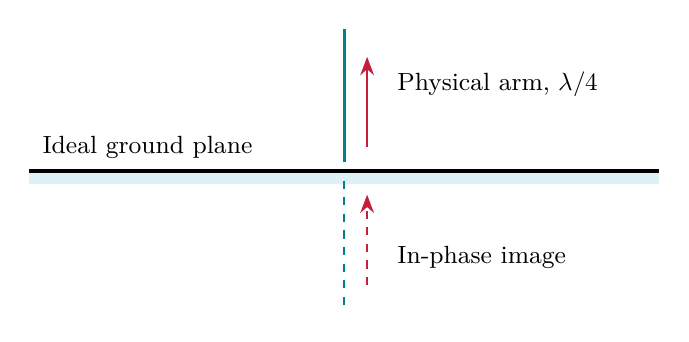
\begin{tikzpicture}[font=\small]
\fill[hdrteal] (-4,-.16) rectangle (4,0);
\draw[very thick] (-4,0)--(4,0);
\draw[very thick,myteal] (0,.12)--(0,1.8);
\draw[thick,myteal,dashed] (0,-.12)--(0,-1.8);
\draw[redarrow] (.29,.3)--(.29,1.45);
\draw[redarrow,dashed] (.29,-1.45)--(.29,-.3);
\node[right] at (.55,1.1) {Physical arm, $\lambda/4$};
\node[right] at (.55,-1.1) {In-phase image};
\node[above] at (-2.5,.03) {Ideal ground plane};
\end{tikzpicture}
\end{tcolorbox}
\begin{itemize}[leftmargin=*,itemsep=3pt]
\item \textbf{Power and resistance.} Same upper field at the same feed current, but half the total radiated power. Hence $R_r\approx36.5\,\Omega$.
\item \textbf{Directivity.} Maximum intensity stays the same while total power halves, so $D_0\approx3.28$ ($5.15\,\mathrm{dBi}$), referenced to a full sphere.
\item \textbf{Applications and limits.} Dipoles can give simple balanced antennas. Monopoles are compact over conductive bodies or radial ground systems. Finite ground, losses and surroundings change impedance and pattern.
\end{itemize}
At $600\,\mathrm{MHz}$ in free space, $\lambda=c/f=0.50\,\mathrm m$. The half-wave dipole is $0.25\,\mathrm m$ end to end with two $0.125\,\mathrm m$ arms. A quarter-wave monopole has one $0.125\,\mathrm m$ arm above ground. Practical tuning adjusts these first estimates.

\section{Past-Paper Extension: Folded Dipole and Arrays}
These applications appeared in a \href{https://www.scribd.com/document/972492704/Electromagnetic-Waves-EC501-5587-I040}{2022--23 EC501 paper} and extend the named topics in Module 5.
\subsection{Folded half-wave dipole}
\begin{tcolorbox}[defbox,title={Folded dipole}]
A folded dipole uses two closely spaced parallel conductors joined at both ends. One conductor is split at its centre for the balanced feed. Its overall span is approximately $\lambda/2$.
\end{tcolorbox}
\begin{tcolorbox}[tikzbox,title={Folded dipole and its in-phase radiation currents},unbreakable]
\centering
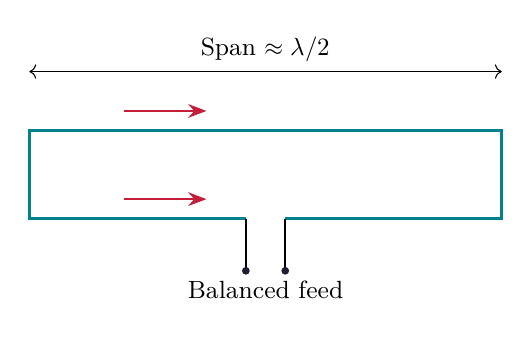
\begin{tikzpicture}[font=\small]
\draw[very thick,myteal] (-.25,0)--(-3,0)--(-3,1.12)--(3,1.12)--(3,0)--(.25,0);
\draw[thick] (-.25,0)--(-.25,-.66) (.25,0)--(.25,-.66);
\fill[mydark] (-.25,-.66) circle (1.4pt) (.25,-.66) circle (1.4pt);
\draw[redarrow] (-1.8,.25)--(-.75,.25);
\draw[redarrow] (-1.8,1.37)--(-.75,1.37);
\node[below] at (0,-.67) {Balanced feed};
\draw[<->] (-3,1.87)--(3,1.87) node[midway,above] {Span $\approx\lambda/2$};
\end{tikzpicture}
\end{tcolorbox}

\begin{enumerate}[leftmargin=*,itemsep=4pt]
\item \textbf{Current and pattern.} For small spacing and equal wire diameters, the in-phase radiation currents have approximately equal half-wave profiles, largest near the centre. Their fields add to give nearly the same normalized pattern as an ordinary half-wave dipole.
\item \textbf{Input resistance.} Near resonance, the folded antenna radiates approximately as an ordinary dipole carrying twice the folded antenna's feed current. At feed current $I$, equate $\tfrac12|I|^2R_{\rm folded}$ with $\tfrac12|2I|^2R_r$. Thus $R_{\rm folded}\approx4R_r\approx292\,\Omega$, often quoted as about $300\,\Omega$. The estimate assumes equal wire diameters, close spacing and negligible loss.
\item \textbf{Bandwidth.} The two-conductor structure alters the input impedance versus frequency and can give a wider usable matching band than a thin single-wire dipole. Actual bandwidth depends on spacing, wire diameter and the VSWR limit.
\end{enumerate}

\subsection{Array factor, broadside and end-fire}
\begin{tcolorbox}[defbox,title={Antenna array}]
An antenna array uses multiple elements whose fields combine in space. Relative excitation amplitudes and phases control the beam direction, beamwidth and sidelobes.
\end{tcolorbox}

Take two identical equally oriented elements at $0$ and $d\hat{\mathbf z}$, each carrying the same current magnitude, with feed phase advance $\delta$ on the second element. Neglect mutual coupling for this pattern calculation. In direction $\theta$ from the array axis the second path is shorter by $d\cos\theta$. With the outgoing phase convention,
\[
\psi=kd\cos\theta+\delta,\qquad
AF=1+e^{j\psi}=2e^{j\psi/2}\cos(\psi/2).
\]
Multiply the element field pattern by $AF$. Power varies as the squared magnitude of the product. With $d=\lambda/4$ and $\delta=0$, the array-factor maximum is at $\theta=90^\circ$ (broadside). With $\delta=-\pi/2$, its maximum occurs at $\theta=0^\circ$ ($+z$ end-fire) and its null is at $\theta=180^\circ$. The element pattern must also permit radiation in the chosen direction.
\begin{itemize}[leftmargin=*,itemsep=3pt]
\item \textbf{Linear array.} Elements lie on a line. A progressive phase controls the beam angle relative to the line.
\item \textbf{Planar and circular arrays.} A planar grid can steer in two angular coordinates. A circular arrangement provides azimuthal symmetry in the geometry and can steer in azimuth.
\item \textbf{Driven and parasitic elements.} Driven elements have a feed. Parasitic elements obtain current by coupling, as in the reflector and directors of a Yagi--Uda antenna.
\end{itemize}

\newpage
\begin{center}
  {\large\bfseries\color{myred} Quick Revision --- Module 5}\\[3pt]
  {\small\color{mydark} Radiation and Antennas $|$ EC501}
\end{center}
\noindent{\color{myred}\rule{\linewidth}{1.2pt}}
\begin{tcolorbox}[formulabox,title={Key Formulas at a Glance}]
\renewcommand{\arraystretch}{1.35}
\begin{tabularx}{\linewidth}{B{5.0cm}Y}
Outgoing kernel & $e^{-jkR}/(4\pi R)$ for time dependence $e^{j\omega t}$ \\[3pt]
Hertzian far field & $E_\theta\approx j\eta k I_0\ell\,e^{-jkr}\sin\theta/(4\pi r)$ \\[3pt]
Radiated power & $\int U\,d\Omega=\eta k^2|I_0\ell|^2/(12\pi)$ for a current element \\[3pt]
Directivity and gain & $D=4\pi U/P_{\rm rad}$, $G=e_r D$ \\[3pt]
Effective aperture & $A_e=\lambda^2G/(4\pi)$ under receive match \\[3pt]
Free-space link & $P_r/P_t=G_tG_r(\lambda/(4\pi R))^2$ for aligned matched link \\[3pt]
\end{tabularx}
\end{tcolorbox}
\begin{tcolorbox}[defbox,title={One-Line Definitions}]
\textbf{Radiation resistance.} Equivalent feed resistance that accounts for power radiated at the specified current.\par
\textbf{Effective aperture.} Available received power divided by incident power flux density for matched polarization.\par
\textbf{Radiation intensity.} Far-zone power radiated per unit solid angle.\par
\end{tcolorbox}
\begin{tcolorbox}[exambox,title={Frequently Asked / Viva Questions}]
\begin{enumerate}[topsep=0pt, label=\textbf{Q\arabic*.}, itemsep=5pt]
\item \Q{Why does the outgoing kernel use a negative phase exponent?}
With $e^{j\omega t}$ it gives a phase moving outward as time increases.
\item \Q{Why keep a position-dependent phase within the source?}
Phase differences between source elements determine the directional far-field pattern.
\item \Q{Which far-field terms carry power to large range?}
The transverse $1/r$ fields supply flux proportional to $1/r^2$.
\item \Q{Where is a Hertzian dipole's pattern null?}
In both directions along its axis.
\item \Q{Why are gain and directivity different?}
Gain includes radiation efficiency.
\item \Q{How does receive polarization tilt affect power?}
Linear tilt by $\psi$ multiplies matched received power by $\cos^2\psi$.
\item \Q{What load maximizes power from a receiving antenna?}
The complex conjugate of its input impedance in the Th\'evenin model.
\item \Q{Why is practical short-dipole radiation resistance smaller?}
Triangular current gives half the current moment of a uniform element at the same feed current and length.
\item \Q{What is the approximate thin half-wave dipole radiation resistance?}
About $73\,\Omega$ in free space.
\item \Q{Why does a quarter-wave monopole have half that resistance?}
At the same current it reproduces the dipole field in half the space and radiates half the total power.
\item \Q{What is the approximate resistance of an equal-wire folded dipole near resonance?}
About $300\,\Omega$, roughly four times that of an ordinary half-wave dipole.
\item \Q{Where do broadside and end-fire arrays point?}
Broadside points perpendicular to the array axis, while end-fire points along it.
\end{enumerate}
\end{tcolorbox}
\begin{tcolorbox}[tikzbox,title={Summary comparison}]
\begin{tabularx}{\linewidth}{|B{4cm}|Y|}\hline
\textbf{Case} & \textbf{What to use} \\ \hline
Hertzian element & Uniform current. Free-space directivity $1.5$. \\ \hline
Half-wave dipole & Approximate sinusoidal current. Directivity $1.64$. \\ \hline
Quarter-wave monopole & Image equivalence over ideal ground. Directivity $3.28$. \\ \hline
\end{tabularx}
\end{tcolorbox}
\end{document}
